\pdfoutput=1
%% Commands for TeXCount
%TC:macro \cite [option:text,text]
%TC:macro \citep [option:text,text]
%TC:macro \citet [option:text,text]
%TC:envir table 0 1
%TC:envir table* 0 1
%TC:envir tabular [ignore] word
%TC:envir displaymath 0 word
%TC:envir math 0 word
%TC:envir comment 0 0
%%
\documentclass[nonacm,sigconf,screen]{acmart} % nonacm to remove all the acm related sections
\settopmatter{printacmref=false} % to remove ACM Reference Format paragraph

% \usepackage{todonotes}
\usepackage{mathtools}
\usepackage{multirow}

%%
%% \BibTeX command to typeset BibTeX logo in the docs
\AtBeginDocument{%
  \providecommand\BibTeX{{%
    Bib\TeX}}}

%% Rights management information.  This information is sent to you
%% when you complete the rights form.  These commands have SAMPLE
%% values in them; it is your responsibility as an author to replace
%% the commands and values with those provided to you when you
%% complete the rights form.
\setcopyright{none}
% \copyrightyear{}
% \acmYear{}
% \acmDOI{}

%% These commands are for a PROCEEDINGS abstract or paper.
% \acmConference[]{}{}{}
%%
%%  Uncomment \acmBooktitle if the title of the proceedings is different
%%  from ``Proceedings of ...''!
%%
%%\acmBooktitle{Woodstock '18: ACM Symposium on Neural Gaze Detection,
%%  June 03--05, 2018, Woodstock, NY}
% \acmISBN{}


%%
%% For managing citations, it is recommended to use bibliography
%% files in BibTeX format.
%%
%% You can then either use BibTeX with the ACM-Reference-Format style,
%% or BibLaTeX with the acmnumeric or acmauthoryear sytles, that include
%% support for advanced citation of software artefact from the
%% biblatex-software package, also separately available on CTAN.
%%
%% Look at the sample-*-biblatex.tex files for templates showcasing
%% the biblatex styles.
%%

%%%%% customised commands
% \renewcommand{\sp}[2]{sp\llbracket#1\rrbracket(#2)}
% \newcommand{\slp}[2]{slp\llbracket#1\rrbracket(#2)}
\newcommand{\slpt}[2]{slp\llbracket#1\rrbracket\big(#2\big)} %slp with tall brackets
% \newcommand{\slpu}[3]{[#1]#2[#3]} % underapproximation triple for slp
% \newcommand{\choice}[2]{\{#1\}\square\{#2\}}
% \newcommand{\ifp}[3]{if (#1) \{#2\} else \{#3\}} % if program, naming because \if is defined and essential
% \newcommand{\while}[2]{while(#1)\{#2\}}
% \newcommand{\incorrectnessP}{\incorrectness} % partial incorrectness

\newcommand{\lemmaautorefname}{Lemma} % for autoref to recognize lemmas

\usepackage{tikz}
\usetikzlibrary{patterns,decorations.pathreplacing,arrows,arrows.meta,decorations.pathmorphing,positioning,fit,trees,shapes,shadows,automata,calc,calligraphy,tikzmark}

% \usepackage{amssymb} % for \mathbb{}
\usepackage{xspace} % needed to work with macros like \Nats

% \usepackage{cleverref}




%
\setlength\unitlength{1mm}
\newcommand{\twodots}{\mathinner {\ldotp \ldotp}}
% bb font symbols
\newcommand{\Rho}{\mathrm{P}}
\newcommand{\Tau}{\mathrm{T}}

\newfont{\bbb}{msbm10 scaled 700}
\newcommand{\CCC}{\mbox{\bbb C}}

\newfont{\bb}{msbm10 scaled 1100}
\newcommand{\CC}{\mbox{\bb C}}
\newcommand{\PP}{\mbox{\bb P}}
\newcommand{\RR}{\mbox{\bb R}}
\newcommand{\QQ}{\mbox{\bb Q}}
\newcommand{\ZZ}{\mbox{\bb Z}}
\newcommand{\FF}{\mbox{\bb F}}
\newcommand{\GG}{\mbox{\bb G}}
\newcommand{\EE}{\mbox{\bb E}}
\newcommand{\NN}{\mbox{\bb N}}
\newcommand{\KK}{\mbox{\bb K}}
\newcommand{\HH}{\mbox{\bb H}}
\newcommand{\SSS}{\mbox{\bb S}}
\newcommand{\UU}{\mbox{\bb U}}
\newcommand{\VV}{\mbox{\bb V}}


\newcommand{\yy}{\mathbbm{y}}
\newcommand{\xx}{\mathbbm{x}}
\newcommand{\zz}{\mathbbm{z}}
\newcommand{\sss}{\mathbbm{s}}
\newcommand{\rr}{\mathbbm{r}}
\newcommand{\pp}{\mathbbm{p}}
\newcommand{\qq}{\mathbbm{q}}
\newcommand{\ww}{\mathbbm{w}}
\newcommand{\hh}{\mathbbm{h}}
\newcommand{\vvv}{\mathbbm{v}}

% Vectors

\newcommand{\av}{{\bf a}}
\newcommand{\bv}{{\bf b}}
\newcommand{\cv}{{\bf c}}
\newcommand{\dv}{{\bf d}}
\newcommand{\ev}{{\bf e}}
\newcommand{\fv}{{\bf f}}
\newcommand{\gv}{{\bf g}}
\newcommand{\hv}{{\bf h}}
\newcommand{\iv}{{\bf i}}
\newcommand{\jv}{{\bf j}}
\newcommand{\kv}{{\bf k}}
\newcommand{\lv}{{\bf l}}
\newcommand{\mv}{{\bf m}}
\newcommand{\nv}{{\bf n}}
\newcommand{\ov}{{\bf o}}
\newcommand{\pv}{{\bf p}}
\newcommand{\qv}{{\bf q}}
\newcommand{\rv}{{\bf r}}
\newcommand{\sv}{{\bf s}}
\newcommand{\tv}{{\bf t}}
\newcommand{\uv}{{\bf u}}
\newcommand{\wv}{{\bf w}}
\newcommand{\vv}{{\bf v}}
\newcommand{\xv}{{\bf x}}
\newcommand{\yv}{{\bf y}}
\newcommand{\zv}{{\bf z}}
\newcommand{\zerov}{{\bf 0}}
\newcommand{\onev}{{\bf 1}}

% Matrices

\newcommand{\Am}{{\bf A}}
\newcommand{\Bm}{{\bf B}}
\newcommand{\Cm}{{\bf C}}
\newcommand{\Dm}{{\bf D}}
\newcommand{\Em}{{\bf E}}
\newcommand{\Fm}{{\bf F}}
\newcommand{\Gm}{{\bf G}}
\newcommand{\Hm}{{\bf H}}
\newcommand{\Id}{{\bf I}}
\newcommand{\Jm}{{\bf J}}
\newcommand{\Km}{{\bf K}}
\newcommand{\Lm}{{\bf L}}
\newcommand{\Mm}{{\bf M}}
\newcommand{\Nm}{{\bf N}}
\newcommand{\Om}{{\bf O}}
\newcommand{\Pm}{{\bf P}}
\newcommand{\Qm}{{\bf Q}}
\newcommand{\Rm}{{\bf R}}
\newcommand{\Sm}{{\bf S}}
\newcommand{\Tm}{{\bf T}}
\newcommand{\Um}{{\bf U}}
\newcommand{\Wm}{{\bf W}}
\newcommand{\Vm}{{\bf V}}
\newcommand{\Xm}{{\bf X}}
\newcommand{\Ym}{{\bf Y}}
\newcommand{\Zm}{{\bf Z}}

% Calligraphic

\newcommand{\Ac}{{\cal A}}
\newcommand{\Bc}{{\cal B}}
\newcommand{\Cc}{{\cal C}}
\newcommand{\Dc}{{\cal D}}
\newcommand{\Ec}{{\cal E}}
\newcommand{\Fc}{{\cal F}}
\newcommand{\Gc}{{\cal G}}
\newcommand{\Hc}{{\cal H}}
\newcommand{\Ic}{{\cal I}}
\newcommand{\Jc}{{\cal J}}
\newcommand{\Kc}{{\cal K}}
\newcommand{\Lc}{{\cal L}}
\newcommand{\Mc}{{\cal M}}
\newcommand{\Nc}{{\cal N}}
\newcommand{\nc}{{\cal n}}
\newcommand{\Oc}{{\cal O}}
\newcommand{\Pc}{{\cal P}}
\newcommand{\Qc}{{\cal Q}}
\newcommand{\Rc}{{\cal R}}
\newcommand{\Sc}{{\cal S}}
\newcommand{\Tc}{{\cal T}}
\newcommand{\Uc}{{\cal U}}
\newcommand{\Wc}{{\cal W}}
\newcommand{\Vc}{{\cal V}}
\newcommand{\Xc}{{\cal X}}
\newcommand{\Yc}{{\cal Y}}
\newcommand{\Zc}{{\cal Z}}

% Bold greek letters

\newcommand{\alphav}{\hbox{\boldmath$\alpha$}}
\newcommand{\betav}{\hbox{\boldmath$\beta$}}
\newcommand{\gammav}{\hbox{\boldmath$\gamma$}}
\newcommand{\deltav}{\hbox{\boldmath$\delta$}}
\newcommand{\etav}{\hbox{\boldmath$\eta$}}
\newcommand{\lambdav}{\hbox{\boldmath$\lambda$}}
\newcommand{\epsilonv}{\hbox{\boldmath$\epsilon$}}
\newcommand{\nuv}{\hbox{\boldmath$\nu$}}
\newcommand{\muv}{\hbox{\boldmath$\mu$}}
\newcommand{\zetav}{\hbox{\boldmath$\zeta$}}
\newcommand{\phiv}{\hbox{\boldmath$\phi$}}
\newcommand{\psiv}{\hbox{\boldmath$\psi$}}
\newcommand{\thetav}{\hbox{\boldmath$\theta$}}
\newcommand{\tauv}{\hbox{\boldmath$\tau$}}
\newcommand{\omegav}{\hbox{\boldmath$\omega$}}
\newcommand{\xiv}{\hbox{\boldmath$\xi$}}
\newcommand{\sigmav}{\hbox{\boldmath$\sigma$}}
\newcommand{\piv}{\hbox{\boldmath$\pi$}}
\newcommand{\rhov}{\hbox{\boldmath$\rho$}}
\newcommand{\upsilonv}{\hbox{\boldmath$\upsilon$}}

\newcommand{\Gammam}{\hbox{\boldmath$\Gamma$}}
\newcommand{\Lambdam}{\hbox{\boldmath$\Lambda$}}
\newcommand{\Deltam}{\hbox{\boldmath$\Delta$}}
\newcommand{\Sigmam}{\hbox{\boldmath$\Sigma$}}
\newcommand{\Phim}{\hbox{\boldmath$\Phi$}}
\newcommand{\Pim}{\hbox{\boldmath$\Pi$}}
\newcommand{\Psim}{\hbox{\boldmath$\Psi$}}
\newcommand{\Thetam}{\hbox{\boldmath$\Theta$}}
\newcommand{\Omegam}{\hbox{\boldmath$\Omega$}}
\newcommand{\Xim}{\hbox{\boldmath$\Xi$}}


% Sans Serif small case

\newcommand{\Gsf}{{\sf G}}

\newcommand{\asf}{{\sf a}}
\newcommand{\bsf}{{\sf b}}
\newcommand{\csf}{{\sf c}}
\newcommand{\dsf}{{\sf d}}
\newcommand{\esf}{{\sf e}}
\newcommand{\fsf}{{\sf f}}
\newcommand{\gsf}{{\sf g}}
\newcommand{\hsf}{{\sf h}}
\newcommand{\isf}{{\sf i}}
\newcommand{\jsf}{{\sf j}}
\newcommand{\ksf}{{\sf k}}
\newcommand{\lsf}{{\sf l}}
\newcommand{\msf}{{\sf m}}
\newcommand{\nsf}{{\sf n}}
\newcommand{\osf}{{\sf o}}
\newcommand{\psf}{{\sf p}}
\newcommand{\qsf}{{\sf q}}
\newcommand{\rsf}{{\sf r}}
\newcommand{\ssf}{{\sf s}}
\newcommand{\tsf}{{\sf t}}
\newcommand{\usf}{{\sf u}}
\newcommand{\wsf}{{\sf w}}
\newcommand{\vsf}{{\sf v}}
\newcommand{\xsf}{{\sf x}}
\newcommand{\ysf}{{\sf y}}
\newcommand{\zsf}{{\sf z}}


% mixed symbols

\newcommand{\sinc}{{\hbox{sinc}}}
\newcommand{\diag}{{\hbox{diag}}}
\renewcommand{\det}{{\hbox{det}}}
\newcommand{\trace}{{\hbox{tr}}}
\newcommand{\sign}{{\hbox{sign}}}
\renewcommand{\arg}{{\hbox{arg}}}
\newcommand{\var}{{\hbox{var}}}
\newcommand{\cov}{{\hbox{cov}}}
\newcommand{\Ei}{{\rm E}_{\rm i}}
\renewcommand{\Re}{{\rm Re}}
\renewcommand{\Im}{{\rm Im}}
\newcommand{\eqdef}{\stackrel{\Delta}{=}}
\newcommand{\defines}{{\,\,\stackrel{\scriptscriptstyle \bigtriangleup}{=}\,\,}}
\newcommand{\<}{\left\langle}
\renewcommand{\>}{\right\rangle}
\newcommand{\herm}{{\sf H}}
\newcommand{\trasp}{{\sf T}}
\newcommand{\transp}{{\sf T}}
\renewcommand{\vec}{{\rm vec}}
\newcommand{\Psf}{{\sf P}}
\newcommand{\SINR}{{\sf SINR}}
\newcommand{\SNR}{{\sf SNR}}
\newcommand{\MMSE}{{\sf MMSE}}
\newcommand{\REF}{{\RED [REF]}}

% Markov chain
\usepackage{stmaryrd} % for \mkv 
\newcommand{\mkv}{-\!\!\!\!\minuso\!\!\!\!-}

% Colors

\newcommand{\RED}{\color[rgb]{1.00,0.10,0.10}}
\newcommand{\BLUE}{\color[rgb]{0,0,0.90}}
\newcommand{\GREEN}{\color[rgb]{0,0.80,0.20}}

%%%%%%%%%%%%%%%%%%%%%%%%%%%%%%%%%%%%%%%%%%
\usepackage{hyperref}
\hypersetup{
    bookmarks=true,         % show bookmarks bar?
    unicode=false,          % non-Latin characters in AcrobatÕs bookmarks
    pdftoolbar=true,        % show AcrobatÕs toolbar?
    pdfmenubar=true,        % show AcrobatÕs menu?
    pdffitwindow=false,     % window fit to page when opened
    pdfstartview={FitH},    % fits the width of the page to the window
%    pdftitle={My title},    % title
%    pdfauthor={Author},     % author
%    pdfsubject={Subject},   % subject of the document
%    pdfcreator={Creator},   % creator of the document
%    pdfproducer={Producer}, % producer of the document
%    pdfkeywords={keyword1} {key2} {key3}, % list of keywords
    pdfnewwindow=true,      % links in new window
    colorlinks=true,       % false: boxed links; true: colored links
    linkcolor=red,          % color of internal links (change box color with linkbordercolor)
    citecolor=green,        % color of links to bibliography
    filecolor=blue,      % color of file links
    urlcolor=blue           % color of external links
}
%%%%%%%%%%%%%%%%%%%%%%%%%%%%%%%%%%%%%%%%%%%


%%
%% end of the preamble, start of the body of the document source.


\begin{document}

%%
%% The "title" command has an optional parameter,
%% allowing the author to define a "short title" to be used in page headers.
\title{Partial Incorrectness Logic}

%%
%% The "author" command and its associated commands are used to define
%% the authors and their affiliations.
%% Of note is the shared affiliation of the first two authors, and the
%% "authornote" and "authornotemark" commands
%% used to denote shared contribution to the research.
\author{Lena Verscht}
% \authornote{Both authors contributed equally to this research.}
% \email{trovato@corporation.com}
% \orcid{1234-5678-9012}
% \author{G.K.M. Tobin}
% \authornotemark[1]
% \email{webmaster@marysville-ohio.com}
\affiliation{%
  \institution{RWTH Aachen}
  %\city{}
  %\state{}
  \country{Germany}
}
\affiliation{%
  \institution{Saarland University}
  %\city{}
  %\state{}
  \country{Germany}
}



\author{{\=A}nr{\'a}n W{\'a}ng}
% \authornote{Both authors contributed equally to this research.}
% \email{trovato@corporation.com}
% \orcid{1234-5678-9012}
% \author{G.K.M. Tobin}
% \authornotemark[1]
% \email{webmaster@marysville-ohio.com}
\affiliation{%
  \institution{Saarland University}
  %\city{}
  %\state{}
  \country{Germany}
}

\author{Benjamin Lucien Kaminski}
% \authornote{Both authors contributed equally to this research.}
% \email{trovato@corporation.com}
% \orcid{1234-5678-9012}
% \author{G.K.M. Tobin}
% \authornotemark[1]
% \email{webmaster@marysville-ohio.com}
\affiliation{%
  \institution{Saarland University}
  %\city{}
  %\state{}
  \country{Germany}
}
\affiliation{%
  \institution{University College London}
  %\city{}
  %\state{}
  \country{United Kingdom}
}



%%
%% By default, the full list of authors will be used in the page
%% headers. Often, this list is too long, and will overlap
%% other information printed in the page headers. This command allows
%% the author to define a more concise list
%% of authors' names for this purpose.
\renewcommand{\shortauthors}{Verscht, W{\'a}ng, Kaminski}

%%
%% The abstract is a short summary of the work to be presented in the
%% article.
% \begin{abstract}
% We investigate \emph{partial incorrectness logic}, a program logic related to O’Hearn's incorrectness logic, analogous to the relationship between partial and total correctness in \emph{Hoare logic} (HL).
% Whereas partial correctness in HL allows divergence, partial \emph{incorrectness} permits unreachability.
% Using Dijkstra’s \emph{predicate transformers}, we examine this duality between divergence and unreachability.
% Further, we provide several examples for applications of partial incorrectness logic.
% \end{abstract}

%%
%% The code below is generated by the tool at http://dl.acm.org/ccs.cfm.
%% Please copy and paste the code instead of the example below.
%%
% \begin{CCSXML}
% \ccsdesc[500]{Do Not Use This Code~Generate the Correct Terms for Your Paper}
% \ccsdesc[300]{Do Not Use This Code~Generate the Correct Terms for Your Paper}
% \ccsdesc{Do Not Use This Code~Generate the Correct Terms for Your Paper}
% \ccsdesc[100]{Do Not Use This Code~Generate the Correct Terms for Your Paper}

%%
%% Keywords. The author(s) should pick words that accurately describe
%% the work being presented. Separate the keywords with commas.
% \keywords{Do, Not, Us, This, Code, Put, the, Correct, Terms, for,
  % Your, Paper}
%% A "teaser" image appears between the author and affiliation
%% information and the body of the document, and typically spans the
%% page.

% \received{20 February 2007}
% \received[revised]{12 March 2009}
% \received[accepted]{5 June 2009}

%%
%% This command processes the author and affiliation and title
%% information and builds the first part of the formatted document.
\maketitle

% \textbf{Workshop website: }\href{https://popl25.sigplan.org/home/tpsa-2025#Call-for-Presentations}{link}.
% \textbf{About formatting: }\href{https://www.sigplan.org/Resources/Author/}{link}.
% \textbf{List of accepted LaTeX packages: }
% \href{https://authors.acm.org/proceedings/production-information/accepted-latex-packages}{link}.

\section{Introduction}
\label{sec:intro}
% correctness and partial correctness
Reasoning about program correctness has been a central topic in static analysis for many years,  with \emph{Hoare logic} (HL) playing an important role~\cite{hoareAxiomaticBasisComputer1969, aptFiftyyearsHoares2019}. %\lv{mehr citations HL?} \awcomment{10 years and 50 years of HL papers?}
The key notions in HL are \emph{partial} and \emph{total correctness}.
Both require that program executions starting in a specified set of initial states (the \emph{precondition}) reach a designated set of final states (the \emph{postcondition}).
Partial correctness is more lenient in that it does not require termination, effectively deeming divergence acceptable.

% incorrectness and topic here: partial incorrectness
We explore \emph{partial incorrectness logic} \cite{zhangQuantitativeStrongestPost2022}, which stands in relation to O'Hearn's \enquote{total} incorrectness logic \cite{ohearnIncorrectnesslogic2020} as partial correctness does to total correctness:
Partial correctness allows divergence, partial \emph{incorrectness} allows \emph{unreachability}.
While the duality between divergence and unreachability may not be immediately apparent, we explore this relationship further.

Our chosen formalism is \emph{predicate transformers} à la Dijkstra~\cite{dijkstraGuardedcommandsnondeterminacy1975}.
We focus here on \emph{deterministic} and \emph{reversible} programs, though the discussion extends to nondeterministic and irreversible computations, both of which introduce additional nondeterminism that must be addressed.

% \lvcommentinline{Ich finde das reicht schon als Intro, vielleicht können wir ein paar Teile noch in die jeweiligen Sections schieben. Was denkst du \ataw}
% \awcomment{Mache gleich. }

% 









\section{Correctness and Termination}
\label{sec:correctness}
Hoare logic \cite{hoareAxiomaticBasisComputer1969} is concerned with triples of the form $\hoare{\pre}{\program}{\post}$, where~$\pre$ is a precondition on initial states, $\program$ is a program, and $\post$ is a postcondition on final states.
$\hoare{\pre}{\program}{\post}$ is said to be \emph{valid for total correctness} if all computations of $\program$ started in initial states satisfying precondition $\pre$ (1) terminate, and (2) do so in some state satisfying the postcondition $\post$.

As is well known, proving termination is undecidable.
This is motivation to define a more lenient notion of correctness, \emph{partial correctness}, which requires only criterion (2) above.
In other words: \emph{If} $\program$ terminates, it has to do so in $\post$.
% In this case, we say that $\hoare{\pre}{\program}{\post}$ is \emph{valid for partial correctness}.

\subsection{Weakest (Liberal) Pre}
\label{ssec:weakestpre}
We use \emph{predicate transformers} due to Dijkstra as the formal framework for expressing program specifications \cite{dijkstraPredicateCalculusProgram1990}.
The \emph{weakest precondition} $\wp{\program}{\post}$ of a postcondition $\post$ with respect to a program~$\program$ contains \emph{all} states from which $\program$ always terminates in $\post$.
Notably, this is the weakest predicate $\pre$ such that $\hoare{\pre}{\program}{\post}$ is valid for \emph{total} correctness.
Dually, the \emph{weakest liberal precondition} $\wlp{\program}{\post}$ of $\post$ with respect to~$\program$ contains \emph{all} states from which $\program$ either diverges or terminates in $\post$.
This is the weakest predicate $\pre$ such that $\hoare{\pre}{\program}{\post}$ is valid for \emph{partial} correctness.

Computing weakest (liberal) preconditions can be done inductively on the program structure.
The most intricate part of this are loops, which require reasoning about fixed points.
The weakest (liberal) preconditions of while loops are defined as fixed points of a characteristic function $\Phi$ which, intuitively, captures one execution of the loop body:
%
% $wp{\WHILEDO\varphi{C'}}{F} \eeq \mu\,\Phi$ and $\wlp{\WHILEDO\varphi{C'}}{F} &\eeq \nu\,\Phi$
%
\begin{align*}
    \wp{\WHILEDO\varphi{C'}}{F} &\eeq \mu\,\Phi\\
    \text{and \qquad } \wlp{\WHILEDO\varphi{C'}}{F} &\eeq \nu\,\Phi~,
\end{align*}%
\noindent%
%
where $\mu\,\Phi$ denotes the least and $\nu\,\Phi$ the greatest fixed point of $\Phi$~\cite{kaminskiAdvancedWeakestPrecondition2019}.
For our intents, the relevant aspect here is that weakest preconditions are \emph{least} fixed points while weakest liberal preconditions are \emph{greatest} fixed points.
% The reason is that: Starting from an initial state satisfying the least fixed point (which is a predicate in our case), the while-program is guaranteed to terminate. 
% Conversely, any initial state that can lead to looping forever, will satisfy the greatest fixed point. 
% \blkin{Den reason kaufe ich so irgendwie nicht ab. Ich würde das streichen. Es ist auch nicht der reason, warum das für uns das einzig relevante ist, oder?}
% \awcomment{Habe nichts dagegen. Erklären wir dann nicht, warum wir wp mit lfp usw. definiert haben? \atlv}
% \lv{Find auch wir können das streichen. Das ist nicht der Grund, wieso das für uns relevant ist (der ist Park's Lemma).}

% \todo[inline]{blk: ich kann der folgenden aufzählung nicht ganz folgen.} 
% \lv{ich verstehe das auch nicht, \ataw kannst du das umschreiben und einbauen oder rausnehmen?}
% \awcomment{Jetzt besser? \atlv at blk}

% In contrast, total correctness is also a lower bound but on a \emph{least} fixed point and there is no similar induction principle to verify candidate lower bounds on least fixed points.
% The reason is that: 
% 1. With least fixed point, termination is guaranteed, i.e. no infinite loop possible. 
% 2. A fixed point that is neither least nor greatest means infinite loop is possible. 
% 3. The greatest fixed point includes all states that can lead to infinite execution. 
% Define function 
% \[\Phi(X):=(\neg\varphi\wedge F)\vee(\varphi\wedge wp.C'.X)\]
% It is often referred to as the characteristic function of the while-loop. 
% wp for while-loop is be defined with least fixed points: 
% \[\wp{\WHILEDO\varphi{C'}}{F} = \mu\Phi(X)\]
% Meanwhile, wlp is defined with greatest fixed points: 
% \[\wlp{\WHILEDO\varphi{C'}}{F} = \nu\Phi(X)\]

% These definitions reflect the underlying semantics of wp and wlp: wp-transformer deems non-termination ``bad'' and wlp-transformer is more liberal about it. 
% By defining wp with least fixed points, we restrict to initial states that guarantee termination, and by defining wlp with greatest fixed points, we expand to all initial states that can lead to non-termination. 
% The postcondition in the wlp setting is guaranteed upon termination.



\subsection{Total and Partial Correctness}
\label{ssec:partialtotalcorr}
Above, we have hinted at the close connection between total (partial) correctness and weakest (liberal) preconditions, which comes as an \emph{underapproximation}:

\noindent
\hspace{-5pt}
% Each can be characterized as an \emph{underapproximation} of a predicate transformer:%
%
% \begin{align*}
%     \hoare{\pre}{\program}{\post} \text{ is valid for total correctness} &\quad \text{iff} \quad \pre \subseteq \wp{\program}{\post}
% \intertext{and}
%     \hoare{\pre}{\program}{\post} \text{ is valid for partial correctness} &\quad \text{iff} \quad \pre \subseteq \wlp{\program}{\post}~.
% \end{align*}%
\begin{tabular}{l|ll}
\multirow{2}{*}{$\hoare{\pre}{\program}{\post}$ is valid for}
     & total correctness \quad &iff \quad $\pre \subseteq \wp{\program}{\post}$ \\
     & partial correctness \quad &iff \quad $\pre \subseteq \wlp{\program}{\post}$ \\
\end{tabular}

For proving total correctness of a loop, we thus have to prove a {lower} bound on a \emph{least} fixed point -- 
for partial correctness, we also have to prove a {lower} bound, but on a \emph{greatest} fixed point.
The latter can be conveniently proven using the following theorem:
% The invariant method to prove correctness can be generalized by Park's lemma. 
% As a corollary of Knaster-Tarski fixed point theorem, Park's induction lets us find upper bounds for least fixed points, and lower bounds for greatest fixed points:%
%
\begin{lemma}[Park Induction]\label{lem:park}
    Let $(X, {\preceq})$ be a complete partial order and $f\colon X \to X$ be monotonic.
    Then for all $I \in X$,%
    %
    \begin{align*}
        % & f(I)\ppreceq I \qimplies \mu f \ppreceq I~, \qquad \textnormal{and} \\
        & I\ppreceq f(I) \qimplies I \ppreceq \nu f.
    \end{align*}%
    %
   % where $\mu$ is the least and $\nu$ is the greatest fixed point operator. 
\end{lemma}%
%
\noindent%
%
%
If we have a suitable candidate or \emph{invariant} $I$, we can thus prove \emph{lower} bounds on \emph{greatest} %and \emph{upper} bounds on \emph{least}
fixed points by just one application of $f$.
For \emph{lower} bounds on \emph{least} fixed points, there is no such simple rule.
The consequence for proofs of correctness is that we can prove partial correctness easily, while total correctness requires more intricate arguments~\cite{harkAimingLowHarder2020}. 

% $I$ is called a \emph{superinvariant} of $f$ if $f(I)\ppreceq I$ and a \emph{subinvariant} of $f$ if $I\ppreceq f(I)$. 
% With Park's induction we can find lower bounds for wlp easily by identifying subinvariants. 
% Then if we can prove that from the states satisfying such a subinvariant, program terminates, then we find also a lower bound of wp, which is not easy (cite "aiming low is hard"?)

\subsection{Termination}
\label{ssec:termination}
% Distinguishing partial and total correctness is only the assessment of termination, which is accepted for partial correctness but forbidden for total correctness. 
% \awcomment{Dieser Satz reformuliert.}
Given a proof of partial correctness, we prove total correctness by additionally proving termination.
% Put symbolically, we have%
% %
% \begin{align*}
%     \text{total correctness} ~{}={}~ \text{partial correctness} + \text{termination}~.
% \end{align*}%
% %
In terms of weakest preconditions, this means
\begin{align*}
    \underbrace{\pre \subseteq \wp{\program}{\post}}_{\text{\scriptsize total correctness}} \quad \impliedby \quad \underbrace{\pre \subseteq \wlp{\program}{\post}}_{\text{\scriptsize partial correctness}} \, \land \, \underbrace{\pre \subseteq \wp{\program}{\true}}_{\text{\scriptsize termination}}.
\end{align*}%
%
Note that we in fact do not require \emph{universal} termination, i.e.\ termination from \emph{all} initial states, but only from the states of interest (those satisfying $\pre$).

There are several reasons why to separate these concerns:
In the spirit of divide and conquer, we can split a problem into smaller subproblems.
Proving partial correctness is indeed conceptually easier than proving total correctness, as we have seen in {\color{ACMPurple}Section}~\ref{ssec:partialtotalcorr}.
Additionally, proving termination is a subfield on its own, meaning we can profit from well developed techniques and algorithms.

% https://teams.microsoft.com/l/meetup-join/19%3ameeting_ZWNkODk5NTAtZDk3MC00NmU3LWEyNjEtMzJlOWM1MjYwMjVm%40thread.v2/0?context=%7b%22Tid%22%3a%2267610027-1ac3-49b6-8641-ccd83ce1b01f%22%2c%22Oid%22%3a%2288f6a93d-2e48-449d-8744-113aefe4cd71%22%7d 

\paragraph{Proving termination using variants}
To prove universal termination%\lv{maybe comment why we do universal termination here and not just of states in b} 
of a while loop $\WHILEDO{\varphi}{\program}$, we can make use of \emph{variants}:
A variant is a function $\variant \colon \states \to \Nats$ such that for all $n \in \Nats$, the triple $\hoare{\varphi\wedge v=n}{\program}{ v<n}$ is valid for total correctness. %\awcomment{frage: v und n haben verschiedene typen, kann man v=n machen?}
Intuitively, each program state is assigned a natural number that has to strictly decrease in every iteration.
Since the natural numbers are well-founded, there cannot be infinitely many iterations.
Therefore, if a variant exists, then the loop $\WHILEDO{\varphi}{\program}$ terminates. %, i.e.\ $\hoare {\true} {\WHILEDO{\varphi}{\program}} {\neg\varphi}$ is valid for total correctness.

% To prove total correctness of a while loop, we can use the well-known \emph{variant} rule: % (we reformulate it to mirror the rule in \ref{ssec:reachability}) 
%Original: \[
%     \frac{\hoare{\pre\wedge\varphi\wedge v=n\wedge v\in\Nats }{\program}{\pre\wedge v<n\wedge v\in\Nats }}
%     {\hoare {\pre\wedge v\in\Nats } {\WHILEDO{\varphi}{\program}} {\neg\varphi\wedge \pre\wedge v\in\Nats }}
% \]
% Regel 0 (b=true):
% \[
%     \frac{\hoare{\varphi\wedge v=n\wedge v\in\Nats }{\program}{v<n\wedge v\in\Nats }}
%     {\hoare {v\in\Nats } {\WHILEDO{\varphi}{\program}} {\neg\varphi\wedge v\in\Nats }}
% \]
% impliziert <b and v in nats > 
% Regel 1: (mit b als invariante)
% \[
%     \frac{v\in\Nats \qquad \hoare{\pre\wedge\varphi\wedge v=n}{\program}{\pre\wedge v<n}}
%     {\hoare {\pre} {\WHILEDO{\varphi}{\program}} {\neg\varphi\wedge \pre}}
% \]
% Regel 2:
% \[
%     \frac{v\in\Nats \qquad \hoare{\varphi\wedge v=n}{\program}{ v<n}}
%     {\hoare {\true} {\WHILEDO{\varphi}{\program}} {\neg\varphi}}
% \]
% Regel 3:
% \[
%     \frac{v\in\Nats \qquad \pre \implies v? \qquad \hoare{\varphi\wedge v=n}{\program}{ v<n}}
%     {\hoare {\pre} {\WHILEDO{\varphi}{\program}} {\neg\varphi}}
% \]
% Regel 4:
% \[
%     \frac{n \in \Nats \quad\quad \hoare{\variant(n+1)\wedge \varphi}{\program}{ \variant(n)}}
%     {\hoare {\exists n\in\Nats .\, \variant(n) } {\WHILEDO{\varphi}{\program}} {\neg\varphi\wedge \variant(0)}}
% \]
% Regel 5:
% \[
%     \frac{\variant \colon \Sigma \to \Nats \qquad n \in \Nats \qquad \hoare{\variant = n \wedge \varphi}{\program}{ \variant < n}}
%     {\hoare {\true } {\WHILEDO{\varphi}{\program}} {\neg\varphi}}
% \]
% It says that if we can find a natural-number-valued variant that decreases with each loop body execution, then we can prove that the program terminates. 
% The term $\variant(n)$ says that we formulate our states of interest as an statement related to some natural number $n$. 
% This statement is valid for a smaller number after the loop body is executed. %\lv{ist nicht $b$ die variant? sollen wir vielleicht um das von pre zu unterscheiden b hier in v umändern (für variant) und das was jetzt v ist in n?}
% Because natural numbers are bounded below by zero, the loop can iterate forever. 
% Consequently, if we can find a witness $n$ that makes $\variant(n)$ valid before the execution of the whole loop, then the loop must terminate. 

% It is necessary to have $n\in\Nats$ as part of the requirement to ensure termination, because otherwise we would be able to prove 
% \[\hoare{x=50}{\WHILEDO{x<0}{x:=x-1}}{x=0}\] 
% which is obviously untrue. 
% Interestingly, this condition is not required in the variant rule for reachability, as we will see in \ref{ssec:reachability}. 
% \lv{schaut gut aus, nur eine kleine frage: braucht man die variante in der conclusion überhaupt? könnte man nicht sagen, dass <true>while<not phi>?}
% \awcomment{Ich bin der Meinung ja braucht man. Ohne dies kann man ``<true> while a>=b $\wedge$ a>0 do a:=a-b <a<b> beweisen mit variant ab, aber wenn b negativ ist, terminiet dieses loop nicht. }
% This rule generalizes to expectations and quantities as well, since they both bounded from above or below by the greatest or the least element of their respective lattice. 
% \blkin{Irgendwie passt diese Regel in Spirit nicht zu dem, was wir oben die ganze Zeit sagen. Denn hier wird ja jetzt die Invariante mit dem Terminierungsbeweis verwurstelt. Ich finde auch nicht gut, dass $b$ jetzt der name für eine invariante ist. vorher war das immer der name der pre. oder verstehe ich was falsch? irgendwas ist aber definitiv durcheinander.}
% \lv{gibt es denn eine variant rule die wirklich nur terminierung beweist \ataw ?
% Also können wir nicht einfach b=true wählen?
% }


\section{Incorrectness and Reachability}
\label{sec:incorrectness}

Reasoning about program correctness is a well-established area of research.
Recently, a dual concept has gained significant attention: program \emph{incorrectness} \cite{ohearnIncorrectnesslogic2020,devriesReverseHoareLogic2011}.
Intuitively, incorrectness is concerned with reachability of a set of final states assumed to represent unwanted behavior, or, \emph{bugs}.
A triple $\incorrectness{\pre}{\program}{\post}$ is valid for incorrectness if all states satisfying $\post$ are reachable via execution of program $\program$ from some initial state in $\pre$.

Similar to correctness, we can also characterize incorrectness as the underapproximation of a predicate transformer.
This raises the question whether for incorrectness we can have a similar separation of concerns as with total correctness in the form of
%
\begin{align*}
    \text{incorrectness} \eeq \text{something} + \text{something else}~.
\end{align*}%
%
We will see that we can answer this positively.
For this, let us again start by looking at the required predicate transformers.


\subsection{Strongest (Liberal) Post}
%\lvcommentinline{hier: what is sp and slp, dual to section 2.1}
%\blkin{ja!}
%They are concerned with the reachability of final states. 
The \emph{strongest postcondition} $\sp{\program}{\pre}$ of a program $\program$ and a precondition $\pre$ contains all \emph{final} states which computation starting from $\pre$ can reach~\cite{dijkstraPredicateCalculusProgram1990}.
% It is the strongest predicate $\post$ such that $\incorrectness{\pre}{\program}{\post}$ is valid for \emph{total} incorrectness.
% Their underapproximation corresponds to (total) incorrectness. 
%
Strongest \emph{liberal} postconditions on the other hand are much less investigated and were only recently introduced by Zhang and Kaminski~\cite{zhangQuantitativeStrongestPost2022}.
%\lv{add cousot reference}\awcomment{which one?\atlv} 
Liberality here refers to permitting unreachability, in contrast to divergence in the correctness setting.
This comes rather natural, because predicate transformers, as other approaches, take a relational view on computation:
In the end, we are not so much interested in what happens within the program, instead, we abstract this to which initial states lead to (or \emph{are related to}) which final states.

\begin{figure}
    \centering
    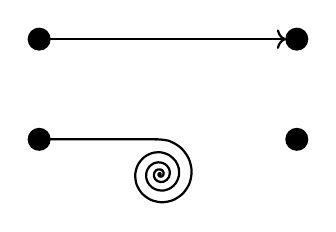
\begin{tikzpicture}[->,
				node distance=1cm and 3cm,
				thick
				]

				\node[state,fill=black,scale=0.3] (I1) {\phantom{1}};
				\node[state,fill=black,scale=0.3] (F1) [right =of I1] {\phantom{1}};
                \node[state,fill=black,scale=0.3] (I2) [below =of I1] {\phantom{1}};
				\node[state,fill=black,scale=0.3] (F2) [right =of I2] {\phantom{1}};

				
				\node (spiral) at ($(I2)!0.5!(F2)$) {};

				\path (I1) edge node {} (F1);
				\path (I2) edge [-] node {} (spiral);

				\coordinate (spiralstart) at ($(spiral)+(-0.1,-0.442)$);
				\draw let \p1=(I2) in
				[scale=0.25,domain=0:30,variable=\t,smooth,samples=75,-,shift={(spiralstart)}] plot  ({\t r}: {-0.002*\t*\t});
			
			\end{tikzpicture}
    \caption{Termination versus reachability.}
    \label{fig:simple-program}
\end{figure}

A simple illustration for this is provided in \autoref{fig:simple-program}.
The program state space only spans two states.
Starting in the first state the program terminates, from the second state the program diverges.
We see that the second initial state from which computation diverges is related to no final state.
Dually, the second final state is related to no initial state; it is \emph{unreachable}. 
%
Therefore, the strongest liberal post $\slp{\program}{\pre}$ contains the states which computation starting from $\pre$ can reach, and additionally the \emph{unreachable states}.
% \blkin{ist das nicht falsch? müssen hier nicht die iwas mit exclusively reachable bla?}
% \lv{ja, im generellen schon. Wir beschränken und auf deterministic reversible programs, dann stimmt das so.}

Similar to weakest (liberal) preconditions, the strongest (liberal) postconditions can be computed using inductive rules.
Those for the $\slpsymbol$ calculus with predicates are given in \autoref{tab:slp-def}. 
% \awcomment{Where to put these footnotes...}\footnote{In \autoref{tab:slp-def}, $\iota \alpha:f$ is the infimum of the function $f$ over all possible values of $\alpha$; $\nu Y.f$ is the greatest fixed point of the function $f$.}

The loop definitions again invoke \emph{least} and \emph{greatest} fixed points of a characteristic function $\Phi$:%
%
\begin{align*}
    &\sp{\WHILEDO\varphi{C'}}{F} = \mu\,\Phi\\ %\quad \text{and } 
    \text{and \qquad } &\slp{\WHILEDO\varphi{C'}}{F} = \nu\,\Phi.
\end{align*}
Again, the liberal calculus corresponds to a \emph{greatest} fixed point and the non-liberal to a \emph{least} fixed point.
%
% Using the least fixed point operator ensures that we only allow reachable states in \spsymbol, and the greatest fixed point operator includes all unreachable states in \slpsymbol.
% \blkin{Auch das sehe ich nicht einfach so immediately ein.}
% \awcomment{Auch wegstreichen oder eine andere Erklärung schreiben? \atlv}
% \lv{ich verstehs auch nicht}
% \awcommentinline{Mit ``lfp = termination'' meine ich \href{http://anran-summary.schuler-christian.de/moc/fixed-point.html}{das hier (link)}. Verstehe ich was falsch?}

\begin{table}
  \renewcommand{\arraystretch}{1.3}
  \begin{tabular}{ll}
    \toprule
    $C$&$\slp{\program}{F}$\\
    \midrule
    $\DIVERGE$ & $\true$\\
    $\ASSIGN{x}{e}$ & $\forall\alpha:x\neq e[x/\alpha]\vee F[x/\alpha]$ \\
    %\footnote{$\iota \alpha:f$ is the infimum of the function $f$ over all possible values of $\alpha$. }\\
    $\COMPOSE{C_1}{C_2}$ & $\slp{C_2}{\slp{C_1}{F}}$\\
    $\ITE{\varphi}{C_1}{C_2}$ & $\slp{C_1}{\neg\varphi\vee F}\wedge \slp{C_2}{\varphi\vee F}$\\
    $\WHILEDO{\varphi}{C'}$ & $\varphi\vee\big(\nu Y.\,F\wedge\slp{C'}{\neg\varphi\vee Y}\big)$ \\
    %\footnote{$\nu Y.f$ is the greatest fixed point of the function $f$.}\\
    % &\footnotesize $\iota \alpha:f$ is the infimum of the function $f$ over all possible values of $\alpha$;
    % $\nu Y.f$ is the greatest fixed point of the function $f$. \\
  \bottomrule
\end{tabular}
  \caption{The strongest liberal postcondition transformer~\cite{zhangQuantitativeStrongestPost2022}}
  \label{tab:slp-def}
\end{table}

\subsection{Total and Partial Incorrectness}
Similar to total correctness, we can characterize \emph{in}correctness as an underapproximation of the \emph{non-liberal} strongest post.
It is thus a natural choice to define a partial variant of incorrectness as an underapproximation of the \emph{liberal} transformer, giving us:

\noindent
\hspace{-5pt}
\begin{tabular}{l|ll}
\multirow{2}{*}{$\incorrectness{\pre}{\program}{\post}$ is valid for}
     & \enquote{total} incorrectness  &iff \ \  $\post \subseteq \sp{\program}{\pre}$ \\
     & partial incorrectness  &iff \ \  $\post \subseteq \slp{\program}{\pre}$ \\
\end{tabular}

% Similar to weakest pre, strongest post is defined with least fixed points, so that only reachable final states are considered. 
% With least fixed point, reachability is guaranteed, i.e. no unreachable states allowed. 
% A fixed point that is neither least nor greatest means some unreachable states may be included. 
% The greatest fixed point includes all unreachable states. 

% Strongest liberal postcondition on the other hand, is less investigated and was only recently defined with soundness proofs by Zhang and Kaminski~\cite{zhangQuantitativeStrongestPost2022}. 
% Dually, partial incorrectness is the underapproximation of the strongest \emph{liberal} postconditions: 
% \[
%     \incorrectness{\pre}{\program}{\post} \text{ is valid for partial incorrectness} \quad \text{iff} \quad \post \subseteq \slp{\program}{\pre}
% \]
For partial incorrectness, $\post$ may contain unreachable states, but \emph{if} a state satisfying $\post$ is reachable, then it was reachable from some initial state satisfying $\pre$.

Using Park induction ({\color{ACMPurple}Lemma}~\ref{lem:park}) again, we can prove partial incorrectness easily (upon finding a suitable invariant).
%\emph{lower} bounds on \slpsymbol, defined via a \emph{greatest} fixed point.
%, and dually \emph{upper} bounds on \spsymbol, which is defined with the \emph{least} fixed points.  
Yet again, proving total incorrectness by finding a lower bound on the non-liberal $\spsymbol$ is hard, which is why we divide this problem into subproblems in the next section.

% partial = slp underapprox
% total = sp underapprox

% Anwendungsbsp partial inc.
% ein gutes und ein schlechtes?


% \begin{table}
%   \caption{Strongest Liberal Postcondition~\cite{zhangQuantitativeStrongestPost2022}}
%   \label{tab:slp-def}
%   \renewcommand{\arraystretch}{1.3}
%   \begin{tabular}{ll}
%     \toprule
%     $C$&$\slp{\program}{f}$\\
%     \midrule
%     $diverge$ & $+\infty$\\
%     $\ASSIGN{x}{e}$ & $\iota\alpha:[x\neq e[x/\alpha]]\curlyvee f[x/\alpha]$\\
%     $C_1;C_2$ & $\slpt{C_2}{\slp{C_1}{f}}$\\
%     $\choice{C_1}{C_2}$ & $\slp{C_1}{f}\curlywedge \slp{C_2}{f}$\\
%     $\ITE{\varphi}{C_1}{C_2}$ & $\slp{C_1}{[\neg\varphi]\curlyvee f}\curlywedge \slp{C_2}{[\varphi]\curlyvee f}$\\
%     $\while{\varphi}{C'}$ & $[\varphi]\curlyvee\big(\nu Y.f\curlywedge\slp{C'}{[\neg\varphi]\curlyvee Y}\big)$\\
%   \bottomrule
% \end{tabular}
% \end{table}


% In \autoref{tab:slp-def}, $\iota \alpha:f$ is the infimum of the function $f$ over all possible values of $\alpha$. 
% $\nu Y.f$ is the greatest fixed point of the function $f$. 

% \begin{lemma}[Soundness of slp~\cite{zhangQuantitativeStrongestPost2022}]
%     $\slp{\program}{\pre}=\lambda \tau.\displaystyle\underset{\sigma:\sigma\to\tau}{\curlywedge} f(\sigma)$
%     % $\slp{\program}{\pre}=\lambda \tau.\iota \sigma: f(\sigma)$
    
%     $\sigma:\sigma\to\tau$ means the $\sigma$'s from where $\tau$ can be reached via $C$.
% \end{lemma}




% \paragraph{Partial Incorrectness Triple}
% \begin{definition}
%     A triple $\slpu{\pre}{\program}{\post}$ is a valid triple for partial incorrectness iff 
%     $$\post\subseteq \slp{\program}{\pre}$$ 
% \end{definition}

% \paragraph{Inference Rules} \todo{Rules for this triple. (may be unnecessary)}



% \paragraph{Invariants}
% As we have seen for correctness, we can apply {\color{ACMPurple}Lemma}~\ref{lem:park} to easily verify lower bounds on greatest fixed points (as we need for partial incorrectness).
% Again, we cannot apply \autoref{lem:park} to verify lower bounds on least fixed points which we would need for proving total incorrectness.


\subsection{Reachability} \label{ssec:reachability}
We can derive partial from total correctness by discharging termination. 
Dually, we obtain partial incorrectness from \enquote{total} incorrectness by discharging reachability.
Reachability is expressible in terms of predicate transformers, very similar as to what we have seen for termination:
\[
    \underbrace{\post \subseteq \sp{\program}{\pre}}_{\text{\scriptsize \enquote{total} incorrectness}} \quad \impliedby \quad \underbrace{\post \subseteq \slp{\program}{\pre}}_{\text{\scriptsize partial incorrectness}} \, \land \, \underbrace{\post \subseteq \sp{\program}{\true}}_{\text{\scriptsize reachability}}.
\]
The strongest post of $\true$ contains all final states that are reachable.
Again, we do not have to require reachability of \emph{all} final states, but only of those in the postcondition $\post$.
% A dual condition stating reachability of all states in $\post$ is $\post \cap \slp{\program}{\false} = \emptyset$.

\paragraph{Proving reachability using variants}
Unreachability is caused by more than loops: 
Even a simple assignment can already introduce unreachable states.
Still, loops remain the most complex part of the reachability proof, as it requires the computation of a fixed point.
Dual to the variant method to prove termination, there are (backward) variant rules to prove reachability~\cite{ohearnIncorrectnesslogic2020, devriesReverseHoareLogic2011}. % (we modify it to mirror the rule in \ref{ssec:termination}).
A function $\variant \colon \states \to \Nats$ is called a \emph{backward variant} if for all $n \in \Nats$, the triple $\incorrectness{v<n \land \varphi}{\program}{v=n}$ is valid for incorrectness.
Intuitively, each state in which the variant has value $n$ must be reachable from a state with value strictly less than $n$.
Again, since the natural numbers are well-founded, there are only finitely many values strictly less than $n$.
Therefore, if a backwards variant $\variant$ exists, then there exists an $n \in \Nats$ such that the states where $\neg\varphi$ holds and $\variant=n$ are reachable when  executing $\WHILEDO{\varphi}{\program}$.
%$\incorrectness {\true} {\WHILEDO{\varphi}{\program}} {\neg\varphi \wedge \variant=n}$ is valid for incorrectness.

Note that this does not prove \emph{universal} reachability, i.e.\ reachability of \emph{all} final states, but only of those where the loop guard does not hold and where the variant takes on value $n$. %\lv{maybe mention that universal reachability for loops does not make any sense anyways}
It would be interesting to see if we can find rules that prove reachability of the states in some postcondition $\post$ only.
% \lv{passe notation an, hier oder bei der termination variant rule, using $\witness$}
% , O'Hearn named it \emph{backward variant} rule~\cite{ohearnIncorrectnesslogic2020}, de Vries and Koutavas call it the while-rule~\cite{devriesReverseHoareLogic2011} 
% Regel 0 (b=true) for termination:
% \[
%     \frac{\hoare{\varphi\wedge v=n\wedge v\in\Nats }{\program}{v<n\wedge v\in\Nats }}
%     {\hoare {v\in\Nats } {\WHILEDO{\varphi}{\program}} {\neg\varphi\wedge v\in\Nats }}
% \]
% Original:
% \[
%     \frac{\incorrectness{\variant(n)\wedge\varphi}{\program}{\variant(n+1)}}
%     {\incorrectness {\variant(0)} {\WHILEDO{\varphi}{\program}} {\neg\varphi\wedge \exists n\in\Nats.\,\variant(n)}}
% \]
% Attempt 1:
% \[
%     \frac{\variant\in\Nats\quad \quad \incorrectness{\variant<n\wedge\varphi}{\program}{\variant=n}}
%     {\incorrectness {\variant=0} {\WHILEDO{\varphi}{\program}} {\neg\varphi\wedge \exists n\in\Nats.\,\variant=n}}
% \]
% Attempt 1.5:
% \[
%     \frac{\incorrectness{\variant\in\Nats \land\variant<n\wedge\varphi}{\program}{\variant\in\Nats \land \variant=n}}
%     {\incorrectness {\variant\in\Nats} {\WHILEDO{\varphi}{\program}} {\variant\in\Nats \land \neg\varphi}}
% \]
% Attempt 2:
% \[
%     \frac{\variant\in\Nats\quad \quad \incorrectness{\variant<n\wedge\varphi}{\program}{\variant=n}}
%     {\incorrectness {true} {\WHILEDO{\varphi}{\program}} {\neg\varphi}}
% \]

% This rule is very similar to natural induction. 
% The condition above is analogous to the inductive step: 
% From $\variant(n)$, via the loop body $\program$, we can reach  $\variant(n+1)$. 
% The conclusion below uses the base case: 
% If $\variant(0)$ is valid, then after the loop execution (at which point $\neg \varphi$ must be satisfied), we must have reached states that make $\variant(n)$ valid for some $n$. 

% As mentioned earlier in \ref{ssec:termination}, we need $n\in\Nats$ as part of the requirement there to ensure termination. 
% Here however, it is not necessary for we do not care about termination. 
% Whenever the loop fails to terminate (loop body $\program$ is executed infinitely often), $\varphi$ is always true and $\neg \varphi \wedge \exists n\in \Nats .\, v(n)$ is always false. 
% Consequently, $\incorrectness{v(0)}{\WHILEDO{\varphi}{\program}}{false}$ is trivially valid for incorrectness. 


% It says that the loop body $\program$ decreases the value of $\witness$, as we backtrack from after its execution to before. 
% If we can find a witness $\witness$, then we can backtrack it through the loop body for $\witness$ times until $\witness$ reaches $0$, at which point we can stop the backtracking for we have found the precondition from which our postcondition can be reached. 
% Then for a final state after the while-loop satisfying the given postcondition, we must be able to backtrack to a state satisfying $\witness=0$, hence this final state is reachable. 
% The reason behind the variant rule for reachability is similar to the variant rule for termination: 
% \[
%     \frac{v\in\Nats \quad \incorrectness{\pre\wedge\varphi\wedge v=n}{\program}{\pre\color{red}\vee\color{black} v<n}}
%     {\incorrectness {\pre} {\WHILEDO{\varphi}{\program}} {\neg\varphi\wedge \pre}}
% \]
% Recall the duality between termination and reachability and our restriction to invertible programs, the triple $\incorrectness{\pre\wedge\varphi\wedge v=n}{\program}{\pre\wedge v<n}$ says that with each loop iteration, we only \emph{reach} states where the variant decreases, and the invariant $\pre$ is, well, invariant. 
% Since $v$ is bounded from below, we can not loop forever to reach states where $v<0$, hence we must reach the states that keep the invariant $b$ and satisfy the loop exit condition $\neg\varphi$. 

% From another perspective, we would like to state that $\varphi\wedge\pre$ is only satisfied by reachable states after the while-loop. 
% Assume we can make some state satisfying $\varphi\wedge\pre$ unreachable. 
% The incorrectness triple $\incorrectness{\pre\wedge\varphi\wedge v=n}{\program}{\pre\wedge v<n}$ makes sure that 

% Note that with incorrectness triples, the weaker the post, the more burden to prove. 
% \awcomment{Rule may be incorrect, change to o'hearn backward variant rule and reference.}
% Above, $\incorrectness{\pre\wedge\varphi\wedge v=n}{\program}{\pre\color{red}\vee\color{black} v<n}$ says that \emph{all} states described by $b\vee v<n$ are reachable. 
% It means that the program $\program$ must do two things: Keep the invariant always satisfied, \emph{and} decrease the variant. 
% % If there were a conjunction in the postcondition, it is then possible that a state satisfying 
% Consequently, all state satisfying $\neg\varphi\wedge\pre$ are reachable via execution of the while-loop. 

% We would like to state that all states satisfying $\neg\varphi\wedge\pre$ are reachable. 
% By contradiction, we assume some state is unreachable. 
% To make a state satisfying $\neg\varphi\wedge v<n$ unreachable, it must have been that loop exit was impossible. 
% However, since the decrement of $v$ is reachable, and $v$ is bound from below, loop exit is then also reachable, we can not make such state satisfying $\neg \varphi$ unreachable. 
% Similarly, since $\pre$ is also always reachable via loop iterations, a state satisfying $\pre$ is then reachable. (??)


\subsection{Partial Incorrectness: Applications}
Beyond serving as a step toward classic (\enquote{total}) incorrectness, partial incorrectness is an interesting property on its own.
We now explore two scenarios where partial incorrectness proves useful.

\paragraph{Underapproximation triples}
Consider the following program inspired by the beginning example of \cite[Section 3.1]{ohearnIncorrectnesslogic2020}:
% \vspace{-1pt}
\[
    p\coloneqq \ITE{x \text{ even}}{\ASSIGN{y}{y+1}}{\ASSIGN{y}{2\cdot y}}
\]
%
% \lv{ne leider nicht. es ginge sowas wie y=y-1, wenn das dann noch sinnvoll ist? Ich versuchs mal zu ändern.}
% \lv{habs, sollte passen jetzt :)}
% \awcomment{Wäre y:=y-1 nicht sinnvoll? Mit ``y:=y+1 else y:=2y'', wenn y=1 pre ist, dann gilt in post y+1=2y. }
Assume the precondition $y=10$ and the postcondition $y=11$.
As \citet{ohearnIncorrectnesslogic2020}, we can now ask:
Is this postcondition an under-approximation of the states reachable by executing $P_y$ starting from the precondition. 
Or equivalently:
Is triple $\incorrectness{y=10}{p}{y=11}$ valid for incorrectness?

It is not.
This seems unintuitive at first.
However, consider a final state where $y=11$ and $x=1$.
This state is unreachable from initial states where $y=10$; in fact, it is entirely unreachable from \emph{any} initial state.
This is because if $x$ is odd, as it is in this example, the final value of $y$ must be even.

This is where \emph{partial} incorrectness logic comes into application.
The triple $\incorrectness{y=10}{p}{y=11}$ \emph{is} valid for partial incorrectness!
Similar to how partial correctness treats divergence as acceptable behaviour, partial incorrectness accepts universal unreachability.
By doing so, we mitigate the cause of the unintuitive scenario encountered before.
\begin{figure}
    \centering
    \begin{align*}
    & \annotate{y=10} \\
    & \IFSYMBOL\,(\, {x \text{ even }} \, )\,\{\, \\
    & \quad \annotate{x \textbf{ odd} \lor y=10} \\
    & \quad \ASSIGN{y}{y+1}  \\
    & \quad \annotate{x \textbf{ odd} \lor  y=11} \\
    & \}\,\ELSESYMBOL\, \{\\
    & \quad \annotate{x \textbf{ even} \lor  y=10} \\
    & \quad \ASSIGN{y}{2 \cdot y} \\
    & \quad \annotate{x \textbf{ even} \lor y \textbf{ odd} \lor y=20} \\
    & \} \\
    & \annotate{(x \textbf{ odd} \lor  y=11) \land (x \textbf{ even} \lor y \textbf{ odd} \lor y=20)}
\end{align*}
\caption{Calculating the strongest liberal post.}
    \label{fig:calc}
\end{figure}


% \awcomment{Ich habe versucht mit y:=2y zu berechnen, aber irgendwas stimmt nicht. \atlv}
% \lv{ja du hast recht, ich schaue morgen nochmal}
% \begin{align*}
%     & \annotate{y=10} \\
%     & \IFSYMBOL\,(\, {x \text{ even }} \, )\,\{\, \\
%     & \quad \annotate{x \textbf{ odd} \lor y=10} \\
%     & \quad \ASSIGN{y}{y+1}  \\
%     & \quad \annotate{x \textbf{ odd} \lor  y=11} \\
%     & \}\,\ELSESYMBOL\, \{\\
%     & \quad \annotate{x \textbf{ even} \lor  y=10} \\
%     & \quad \ASSIGN{y}{2y} \\
%     & \quad \annotate{x \textbf{ even} \lor  y=20} \\
%     & \} \\
%     & \annotate{(x \textbf{ odd} \lor y=11) \land (x \textbf{ even} \lor  y=20)}
% \end{align*}

Formally, we can prove the validity of the triple for partial correctness by calculating $\slp{p}{y=10}$, which is done by applying the rules presented in \autoref{tab:slp-def}.
Detailed calculations are shown in \autoref{fig:calc}.
Since the postcondition $y=11$ implies $\slp{p}{y=10} = (x \text{ odd } \lor  y=11) \land (x \text{ even } \lor y \text{ odd} \lor y=20)$, the above triple is valid for partial incorrectness.
Thus, partial incorrectness can help focus the reasoning on variables of interest.

% \paragraph{Fairness}
% In the spirit of \cite{devriesReverseHoareLogic2011}, we can use partial incorrectness to provide specifications for the correctness of algorithms.
% Say we are interested in evaluating an algorithm $P_{\text{assign}}$ which assigns students to classes.
% We want to make sure that each class is either assigned no student at all (i.e.\ this class is unreachable), or at least one female student.
% This can be expressed by the partial incorrectness triple $\incorrectness{\text{student is female}}{P_{\text{assign}}}{\text{true}}$.

% Consider an algorithm which assigns elements to five groups or classes.
% Say the elements in question have some internal property and they either belong to group 1 or group 2.
% I want to prevent discrimination of group 1.
% For that purpose, I want to make sure that whenever a class can be reached, then it can be reached from group 1.
% It is fine, however, if a class cannot be reached at all.
% My partial incorrectness triple is:
% <group 1> algorithm <true>

\paragraph{Backtracking responsibilities} 
With partial incorrectness triples in the form of $\incorrectness{\_}{\program}{\text{true}}$, we can reason about responsibilities:
The blank can be filled by initial states that are responsible for some result.
Consider Schrödinger's cat sitting in a sealed box, described by the program $\program:= \WHILEDO{\neg \open}{\ASSIGN{\dead}{\spill}};\  \ASSIGN{\dead}{\spill}$. 
The cat may or may not be $\dead$ depending on whether a vial of poison was $\spill$ed. %\lv{typesetting wie im program -> macro?}
Once we $\open$ the box, we observe the cat's health. % and describe it in the postcondition. 
If we do not open the box, the variable $\dead$ may be true or false at any time, but we have no observations. 
% We model this with a while-loop.  
% we can not assign any value to the cat, so we do not reach any final state, which we model with $\DIVERGE$: 
% \[
% \program:= \ITE{open}{\ASSIGN{dead}{spill}}{\DIVERGE}
% \]
% \[
% \]
% \begin{align*}
%     & \WHILE{\neg open} \\
%     & \quad \ASSIGN{dead}{spill}  \\
%     & \}; \\
%     & \ASSIGN{dead}{spill} \\
% \end{align*}
% \lv{The calculations check out. I am just a bit confused why the diverge statement is there. Maybe the intention of this can be explained as well?}
% \begin{align*}
%     & \annotate{\textbf{open}} \\
%     & \IFSYMBOL\,(\, {\text{open}} \, )\,\{\, \\
%     & \quad \annotate{\neg \textbf{open} \vee \textbf{open}} \\
%     & \quad \ASSIGN{\text{dead}}{\text{spill}}  \\
%     & \quad \annotate{\textbf{true} \vee \textbf{dead} \neq \textbf{spill} } \\
%     & \}\,\ELSESYMBOL\, \{\\
%     & \quad \annotate{\textbf{open} \vee \textbf{open}} \\
%     & \quad \DIVERGE \\
%     & \quad \annotate{\textbf{true}} \\
%     & \} \\
%     & \annotate{\textbf{true}}
% \end{align*}
% \lv{ich denke auch, wir haben ja schon eine genaue berechnung von slp in beispiel 1. vielleicht reicht hier die intuition für das tripel?}

Here, $\incorrectness{\open}{\program}{\true}$ is a valid partial incorrectness triple. 
The postcondition $\true$ tells us that any reachable final state must have an origin satisfying $\open$:
The action of opening the box caused us to have knowledge over the cat. 

Similar reasoning can be acquired by \emph{total} incorrectness.
However, this is subject to the strong condition that there are no unreachable states at all.
For this example, $\incorrectness{\text{open}}{\program}{\text{true}}$ is indeed invalid for total incorrectness.
% \awcomment{rewritten. but true as post is really specific. can it be relaxed? }
% The same can not be achieved with total incorrectness: A valid total incorrectness triple for this example is $\incorrectness{open}{\program}{open \wedge dead=spill}$. 
% We gain from this triple the knowledge of where initially $open$ will take us, but do not know whether the action of opening the box is required for us to make progress. \awcomment{rewrite}

% Assume we have multiple processes all attempting to enter a critical section, then with a valid incorrectness triple $\incorrectness{readyA}{\program}{critA}$ we can prove fairness in the sense that if process $A$ is ready to enter the critical section, then eventually it will. 
% : $\incorrectness{readyA}{\program}{critA}$ for partial incorrectness proves that \emph{if} $A$ entered critical section, then it must be from its own will, not forced by some other process. 
% Yet here we have no guarantee that $A$ will enter the critical section. 

% Rewriting Peterson's mutual exclusion protocol \awcomment{Cite}, we have the following program: 
% \begin{align*}
%     & \annotate{[readyA]} \\
%     & \quad \ASSIGN{turn}{B}  \\
%     & \quad \annotate{[turn\neq B\vee readyA]} \\
%     & \quad \annotate{[readyA] \text{ (consequence rule) }} \\
%     & \WHILE{readyB \wedge turn = B} \\
%     & \quad \annotate{[readyA] \text{ (assume other processes do not temper with $readyA$) }} \\
%     & \quad wait() \\
%     & \quad \annotate{[readyA]} \\
%     & \}\\
%     & \annotate{[readyB\wedge turn=B\vee readyA]} \\
%     & \annotate{[readyA]} \\
%     & \quad \ASSIGN{critA}{true}  \\
%     & \annotate{[\neg critA \vee readyA]} \\
% \end{align*}





% \paragraph{Differential Privacy} 
% Informally, differential privacy is upheld, if observations from two marginally different inputs can not be distinguished. 
% Suppose we have two variables, variable $x$ whose value we wish to keep private and variable $y$ which we allow to be observed in some form.
% Take as an example the program: 
% $$C:=\ITE{x\%3}{y:=1}{y:=0}$$ 
% If we allow direct observation over $y$, we can infer whether $x$ is modulo $3$ depending on the final value of $y$, either $1$ or $0$, see \autoref{fig:example-privacy}. 



% \begin{figure}
%   \centering
%   \includegraphics[width=\linewidth]{images/example-privacy.png}
%   \caption{An example about differential privacy.}
%   \label{fig:example-privacy}
%   \Description{Calculation of $\slp{\program}{x}$ where $x$ is a private variable.}
% \end{figure}

% \begin{align*}
%     & \annotate{[x]} \\
%     & \IFSYMBOL\,(\, {x \% 3} \, )\,\{\, \\
%     & \quad \annotate{\neg x \% 3 \ccurlyvee x} \\
%     & \quad \ASSIGN{y}{1}  \\
%     & \quad \annotate{[y\neq 1]\ccurlyvee [\neg x\%3] \ccurlyvee x} \\
%     & \}\,\ELSESYMBOL\, \{\\
%     & \quad \annotate{[x \%3] \ccurlyvee x} \\
%     & \quad \ASSIGN{y}{0} \\
%     & \quad \annotate{[y \neq 0] \ccurlyvee [x\%3] \ccurlyvee x} \\
%     & \} \\
%     & \annotate{x \text{ odd or } y=12}
% \end{align*}

% Instead, if we allow the indirect observation, namely an partial incorrectness underapproximation triple $\slpu{\pre}{\program}{x}$, the same inference can not be made: $\slpu{x}{\program}{17}$ is a valid triple (in fact, any number in place of $17$ would suffice), yet without knowing the reachability of final states where $\sigma(x)=17$, we can not infer the value of $x$. 
% The same effect can not be achieved using an underapproximation of $\sp{\program}{x}$, because we would have $-\infty$ replacing $\infty$, whence by observing a valid underapproximation triple where $\alpha\preceq\sp{\program}{x}$, we know that the real value of $x$ is $\alpha$, which we do not desire. 
% With the earlier valid partial incorrectness triple, if we know whether final states where the value of $x$ equals $17$ are reachable, then $\slpu{x}{\program}{17}$ is also valid for total incorrectness, and we can infer the initial value of the private variable $x$. 



\section{Conclusion}
\label{sec:conclusion}
We discussed the relatively unexplored notion of partial incorrectness.
In doing so, we stressed the duality between the weakest (liberal) pre and strongest (liberal) post; correctness and incorrectness; termination and reachability.
% We point out that correctness and termination go together, incorrectness and reachability are a couple, and not the other way around.
We argue that partial incorrectness also proves useful in computational terms, as does partial correctness: 
Park's induction allows simple proofs of \emph{partial} incorrectness but not of \emph{total} incorrectness.
By adding a proof of reachability, we can get from partial to total incorrectness.

The examples show that partial incorrectness allows us to drop irrelevant variables and reason about responsibilities.
Further applications for partial incorrectness are still open to investigation.

% \awcomment{Falls die Absätze unnötig sind, einfach löschen\atlv}

% \paragraph{Extending to non-deterministic and non-reversible programs}
% In this talk, we restricted our program to non-deterministic and non-reversible ones for demonstration purposes, but they need not be. 
% When allowing either, we must address the resulting nondeterminism. % and choose an angelic or demonic resolution.


\paragraph{Quantitative programs}
For simplicity, we chose the pre and post to be Boolean predicates. 
However, techniques mentioned here extend to quantitative \emph{expectations} \cite{morgan1996probabilistic,kaminskiAdvancedWeakestPrecondition2019} and we conjecture that the results transfer.

\paragraph{Proving reachability}
We presented a variant rule for proving reachability of loops.
However, assignments can also cause unreachability, and their computation is not straightforward; efficient methods for this would be valuable to investigate.
% Methods for proving termination have been extensively researched.
% It would be interesting to explore whether these techniques can be adapted to reachability.
%To the best of our knowledge, little research has focused on proving reachability, especially in comparison to termination.


\paragraph{Nomenclature}
We feel that the names ``correctness'' and ``incorrectness'' are not covering the entire range of applications of the logics. %\lv{vielleicht den absatz streichen}
Certainly, when we choose the postcondition to represent bugs, we reason about unwanted properties of our programs, but as is shown in our examples, we can just as well analyse properties where the post represents desirable final states.
% What other scenarios are suitable?
% Is there a more suitable name?
% These questions are worth investigating. 

% \paragraph{Variant is for both termination and reachability}
% To prove termination, we reason that the loop body decreases some $\Nats$-valued variable as we go forward, but for reachability, we move backwards to see how our variant was increased by the loop body. 


% \todo{make sure above is qualitative} -> done

% \section{Appendices}


%%
%% The acknowledgments section is defined using the "acks" environment
%% (and NOT an unnumbered section). This ensures the proper
%% identification of the section in the article metadata, and the
%% consistent spelling of the heading.
% \begin{acks}
% To Robert, for the bagels and explaining CMYK and color spaces.
% \end{acks}

%%
%% The next two lines define the bibliography style to be used, and
%% the bibliography file.
\bibliographystyle{ACM-Reference-Format}
\bibliography{__references}
% \awcomment{clean reference entries}

%%
%% If your work has an appendix, this is the place to put it.
% \appendix
% \section{Appendix}

\end{document}
\endinput
%%
%% End of file `sample-sigconf.tex'.






%%%% find a spot for these
As the last chapter of their book~\cite{dijkstraPredicateCalculusProgram1990}, Dijkstra and Scholten introduced the strongest postcondition transformer (sp) as a supplement for the precondition transformers, to describe reachable final states. 
% Some work developed from this postcondition calculus, for example, de Vries and Koutavas~\cite{devriesReverseHoareLogic2011} use \spsymbol to express post-specifications about randomized algorithms, although they called it \emph{reverse Hoare logic}.
% %, the reason of which we conjecture is their angelic resolution of the non-determinism. 
% More recently, O'Hearn~\cite{ohearnIncorrectnesslogic2020} uses \spsymbol to construct \emph{incorrectness logic} by underapproximating it, building a new method to statically analyse errors in programs. 
% Zhang and Kaminski~\cite{zhangQuantitativeStrongestPost2022} coined this system \emph{total} incorrectness logic, in the sense that the post must always be \emph{reachable}.

% \todo{Elaborate on incorrectness logic}


% Analogous to the couple weakest precondition (wp) and weakest \emph{liberal} precondition (wlp), which differ from liberal and non-liberal treatment of termination, \spsymbol and strongest \emph{liberal} postcondition (slp) are also a couple in a similar sense. 
% With wp and wlp, the latter takes a liberal view over \emph{termination}, hence allowing initial states that lead to non-termination to satisfy wlp of some postcondition. 
% When it comes to postconditions, various articles are also concerned with termination, using the word ``liberal'' in the name \slpsymbol to refer to the view on termination~\cite{wuSemanticswlpslp2011, jacobsGeneralcorrectnessunification1985, wulandariVerifyingGraphPrograms2020}. 

% We argue that it is more appropriate to reason about \emph{reachability} instead of termination with respect to post transformers, like other work do~\cite{dijkstraPredicateCalculusProgram1990, zhangQuantitativeStrongestPost2022, ohearnIncorrectnesslogic2020}, because of the dualities we illustrate in the upcoming sections. 
% Zhang and Kaminski~\cite{zhangQuantitativeStrongestPost2022} defined \slpsymbol as a post transformer that deems unreachable final states ``good'' and accepted, and gave soundness proofs with collecting semantics, which to our knowledge is a first. 

% \awcomment{Remove?}
% \paragraph{Why Liberal} Consider program $x:=1;y:=2$. We would like to anticipate the value of $y$, but strongest post transformers give us only the reachable states, and there must be restrictions over $x$, which in this case is irrelevant to us. 
% Conversely, strongest liberal post transformers by construction includes unreachable states, in this case for example, an unreachable state where both $x$ and $y$ have value $2$. 
% slp allows us to drop irrelevant information if we only inquire about part of the variables in the program. 
% If we wish to eliminate unreachable states with the addition of some reachability proof, we end up with \spsymbol transformers from \slpsymbol transformers: $slp+reachability=sp$. 

